\chapter {Fase I: Análisis}
\label{cap:Fase I. Análisis}

Medicina y Tecnología han caminado juntas desde el principio de los tiempos: desde el instrumental quirúrgico y su evolución a lo largo de los siglos, pasando por el fonendoscopio, las prótesis, el electrocardiograma, las radiografías o la resonancia magnética. Son muchos los avances tecnológicos que han facilitado la labor de los médicos a la hora de emitir diagnósticos y aplicar tratamientos.
\textbf{\textcolor{red}{\huge PENDIENTE}}


\section{Predicción del RCV de Framingham}

\begin{figure}[htb]
	\centering
	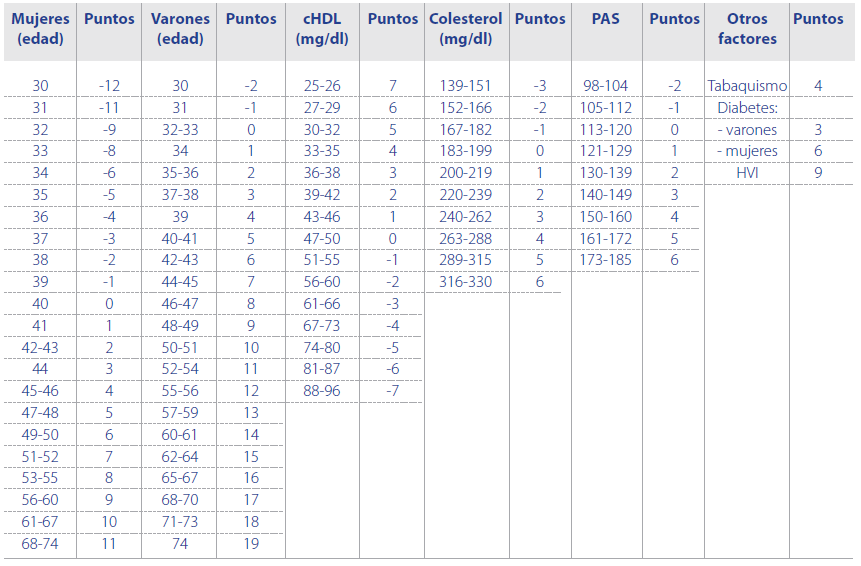
\includegraphics[width=\textwidth]{tablaFir} 
	\caption[Tabla Framighan]{Tabla de Predicción del RCV de Framingham (Anderson, 1991) \cite{tagle2007estimacion}
	}
	\label{fig:tablaFir1}
\end{figure}

\begin{figure}[htb]
	\centering
	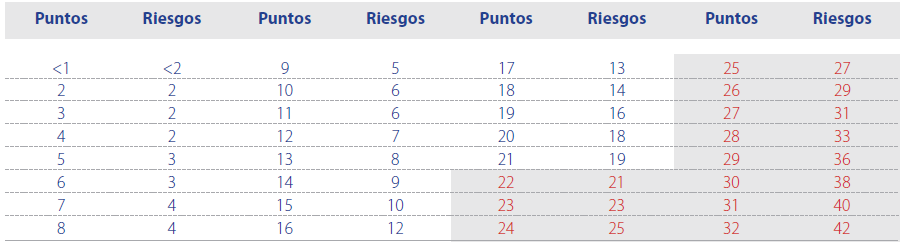
\includegraphics[width=\textwidth]{tablaFir2} 
	\caption[Predicción Framighan]{Predicción del RCV de Framingham (Anderson, 1991) \cite{tagle2007estimacion}
	}
	\label{fig:tablaFir2}
\end{figure}